\documentclass[a4paper,14pt]{extarticle}

% Кодировка и русский язык
\usepackage[T2A]{fontenc}
\usepackage[utf8]{inputenc}
\usepackage[russian]{babel}

% Поля и оформление
\usepackage[left=30mm,right=15mm,top=20mm,bottom=20mm]{geometry}
\usepackage{amsmath,amssymb}
\usepackage{graphicx}
\usepackage{float}
\usepackage{booktabs,array}
\usepackage{indentfirst}
\usepackage{caption}
\usepackage[hidelinks]{hyperref}

\setlength{\parindent}{1.25cm}
\setlength{\parskip}{0pt}
\linespread{1.08}
\renewcommand{\arraystretch}{1.15}

\begin{document}

% ==================== ТИТУЛЬНЫЙ ЛИСТ ====================
\begin{titlepage}
    \centering
    {\large Московский Физико-Технический Институт\par}

    \vspace{4cm}

    {\Large Лабораторная работа № 3.7.3\par}
    \vspace{0.7cm}
    \rule{\textwidth}{0.5pt}\par
    \vspace{0.35cm}
    {\LARGE\bfseries Длинные линии\par}
    \vspace{0.35cm}
    \rule{\textwidth}{0.5pt}\par

    \vfill

    \vspace{6.1cm}
\hfill
\begin{minipage}{0.42\textwidth}
  \raggedright
  Выполнил:\\
  Студент 2 курса ФАКТ\\
  Группа Б03-502\\
  Подмосковнов Лев
\end{minipage}

    \vfill
    {Долгопрудный --- 2026\par}
\end{titlepage}

% ==================== ЦЕЛЬ И ОБОРУДОВАНИЕ ====================
\section{Цель работы}
Исследовать распространение электрических сигналов вдоль длинной линии,
измерить амплитудно-частотную и фазово-частотную характеристики
коаксиального кабеля, определить его погонные параметры и изучить
распределение амплитуды колебаний в модели длинной линии.

\section{Оборудование}
Осциллограф АКТАКОМ ADS-6142H, генератор АКИП 3420/1, коаксиальный
кабель РК-50-4-11, модель длинной линии, магазин сопротивлений Р33,
соединительные провода.

% ==================== ТЕОРИЯ ====================
\section{Теоретическое введение}

Для длинной линии в СГС телеграфные уравнения имеют вид
\begin{equation}
    \begin{cases}
        \displaystyle \frac{\partial I}{\partial x}
            =-C_x\frac{\partial U}{\partial t},\\[2mm]
        \displaystyle \frac{\partial U}{\partial x}
            =-\frac{L_x}{c^2}\frac{\partial I}{\partial t}-R_x I.
    \end{cases}
\end{equation}

Фазовая скорость и волновое сопротивление при малом затухании:
\begin{equation}
    V_{\text{ф}}=\frac{c}{\sqrt{L_x C_x}},
    \qquad
    Z_0=\frac{1}{c}\sqrt{\frac{L_x}{C_x}}.
\end{equation}

Для согласованной нагрузки отражённая волна отсутствует. Амплитуда
и набег фазы на выходе линии длиной $l$ определяются выражениями
\begin{equation}
    U_{\text{н}}=U_0e^{-\alpha l},
    \qquad
    \Delta\varphi=kl,
    \qquad
    k=\frac{\omega}{V_{\text{ф}}},
    \qquad \omega=2\pi\nu.
\end{equation}

Из экспериментальных данных:
\begin{equation}
    \alpha(\omega)=\frac{1}{l}\ln\frac{U_0}{U_{\text{н}}},
    \qquad
    k(\omega)=\frac{\Delta\varphi}{l}.
\end{equation}

При обработке ФЧХ необходимо учитывать полный набег фазы:
\begin{equation}
    \Delta\varphi=2\pi\nu\Delta t+2\pi m,
    \qquad m=0,1,2,\ldots
\end{equation}

% ==================== ЧАСТЬ I ====================
\section{Оценка фазовой и групповой скоростей}

\subsection{Синусоидальный сигнал. Согласованная линия}
При нагрузке $R_{\text{н}}=50\,\text{Ом}$ измерены резонансные частоты,
соответствующие набегу фазы $\Delta\varphi=2\pi n$.

\begin{table}[H]
    \centering
    \caption{Резонансные частоты для согласованной линии}
    \begin{tabular}{ccccccccc}
        \toprule
        $n$ & 1 & 2 & 3 & 4 & 5 & 6 & 7 & 8\\
        \midrule
        $\nu_n$, МГц & 3,85 & 7,8 & 11,8 & 15,8 & 19,8 & 23,3 & 27,1 & 31,2\\
        \bottomrule
    \end{tabular}
\end{table}

Из зависимости $\nu_n(n)$ определим фазовую скорость:
\begin{equation}
    V_{\text{ф}} = l\frac{\Delta \nu}{\Delta n}
    = 50{,}085 \cdot
    \frac{31{,}2 - 3{,}85}{8 - 1} \cdot 10^6
    \approx 1{,}96 \cdot 10^8 \ \text{м/с}.
\end{equation}

Зависимость резонансной частоты от номера резонанса
приблизительно линейна. Следовательно, заметная
дисперсия в исследованном диапазоне частот отсутствует.

\subsection{Синусоидальный сигнал. Линия без нагрузки}
При $R_{\text{н}}=1\,\text{МОм}$ измерены следующие резонансные частоты:

\begin{table}[H]
    \centering
    \caption{Резонансные частоты для разомкнутой линии}
    \begin{tabular}{ccccccccc}
        \toprule
        $n$ & 1 & 2 & 3 & 4 & 5 & 6 & 7 & 8\\
        \midrule
        $\nu_n$, МГц & 3,8 & 7,8 & 11,2 & 15,1 & 19,1 & 23,0 & 27,0 & 31,0\\
        \bottomrule
    \end{tabular}
\end{table}

Из зависимости $\nu_n(n)$ определим фазовую скорость:
\begin{equation}
    V_{\text{ф}} = l\frac{\Delta \nu}{\Delta n}
    = 50{,}085 \cdot
    \frac{31{,}0 - 3{,}8}{8 - 1} \cdot 10^6
    \approx 1{,}95 \cdot 10^8 \ \text{м/с}.
\end{equation}

Полученная фазовая скорость отличается от значения
для согласованной линии примерно на $0{,}55\%$.
Следовательно, наличие или отсутствие согласованной
нагрузки практически не влияет на фазовую скорость
распространения сигнала.

\subsection{Прямоугольные импульсы. Согласованная линия}
В режиме согласованной нагрузки по резонансным частотам повторения
импульсов оценивается групповая скорость.

\begin{table}[H]
    \centering
    \caption{Резонансные частоты для импульсов при согласованной нагрузке}
    \begin{tabular}{cccccc}
        \toprule
        $n$ & 1 & 2 & 3 & 4 & 5\\
        \midrule
        $\nu_n$, МГц & 3,9 & 7,8 & 11,7 & 15,6 & 19,5\\
        \bottomrule
    \end{tabular}
\end{table}

Из зависимости $\nu_n(n)$ определим групповую скорость:
\begin{equation}
    V_{\text{гр}} = l\frac{\Delta \nu}{\Delta n}
    = 50{,}085 \cdot
    \frac{19{,}5 - 3{,}9}{5 - 1} \cdot 10^6
    \approx 1{,}95 \cdot 10^8 \ \text{м/с}.
\end{equation}

Групповая скорость практически совпадает с фазовой
скоростью $V_{\text{ф}} \approx 1{,}96 \cdot 10^8$ м/с.
Следовательно, заметная дисперсия в исследованном
диапазоне частот отсутствует.

\subsection{Прямоугольные импульсы. Линия без нагрузки}
\begin{table}[H]
    \centering
    \caption{Резонансные частоты импульсов при разомкнутой линии}
    \begin{tabular}{cccccc}
        \toprule
        $n$ & 1 & 2 & 3 & 4 & 5\\
        \midrule
        $\nu_n$, МГц & 3,88 & 7,82 & 11,76 & 15,7 & 19,65\\
        \bottomrule
    \end{tabular}
\end{table}

Из зависимости $\nu_n(n)$ определим групповую скорость:
\begin{equation}
    V_{\text{гр}} = l\frac{\Delta \nu}{\Delta n}
    = 50{,}085 \cdot
    \frac{19{,}65 - 3{,}88}{5 - 1} \cdot 10^6
    \approx 1{,}97 \cdot 10^8 \ \text{м/с}.
\end{equation}

Полученная групповая скорость отличается от значения
для согласованной линии примерно на $1{,}1\%$.
Следовательно, наличие или отсутствие согласованной
нагрузки практически не влияет на групповую скорость.
Заметная дисперсия отсутствует.

\newpage

% ==================== ЧАСТЬ II ====================
\section{Амплитудно-частотная и фазово-частотная характеристики}

При согласованной нагрузке $50\,\text{Ом}$ в диапазоне
$1$--$40\,\text{МГц}$ измерены амплитуды напряжения на входе
и выходе и временной сдвиг сигналов.

\begin{table}[H]
    \centering
    \caption{Экспериментальные данные для АЧХ и ФЧХ}
    \small
    \setlength{\tabcolsep}{7pt}
    \renewcommand{\arraystretch}{1.15}
    \begin{tabular}{cccccc}
        \toprule
        $\nu$, МГц & $U_0$, мВ & $U_{\text{н}}$, мВ
        & $\Delta t$, нс & $\Delta\varphi$, рад & $m$ \\
        \midrule
        1  & 27,8 & 26,0 & 252 & 1,58  & 0  \\
        4  & 28,0 & 26,0 & 7   & 6,46  & 1  \\
        7  & 27,6 & 24,6 & 31  & 11,20 & 2  \\
        11 & 29,0 & 25,2 & 12  & 18,02 & 3  \\
        20 & 28,4 & 21,8 & 5,4 & 32,09 & 5  \\
        25 & 27,2 & 19,0 & 15  & 40,06 & 6  \\
        30 & 26,6 & 18,5 & 12  & 48,00 & 8  \\
        35 & 26,6 & 17,3 & 3,2 & 55,85 & 9  \\
        40 & 26,1 & 17,3 & 4,6 & 63,99 & 10 \\
        \bottomrule
    \end{tabular}
\end{table}

По экспериментальным данным построим амплитудно-частотную
характеристику длинной линии:
\begin{equation}
    A(\nu) = \frac{U_{\text{н}}}{U_0}.
\end{equation}

\begin{figure}[H]
    \centering
    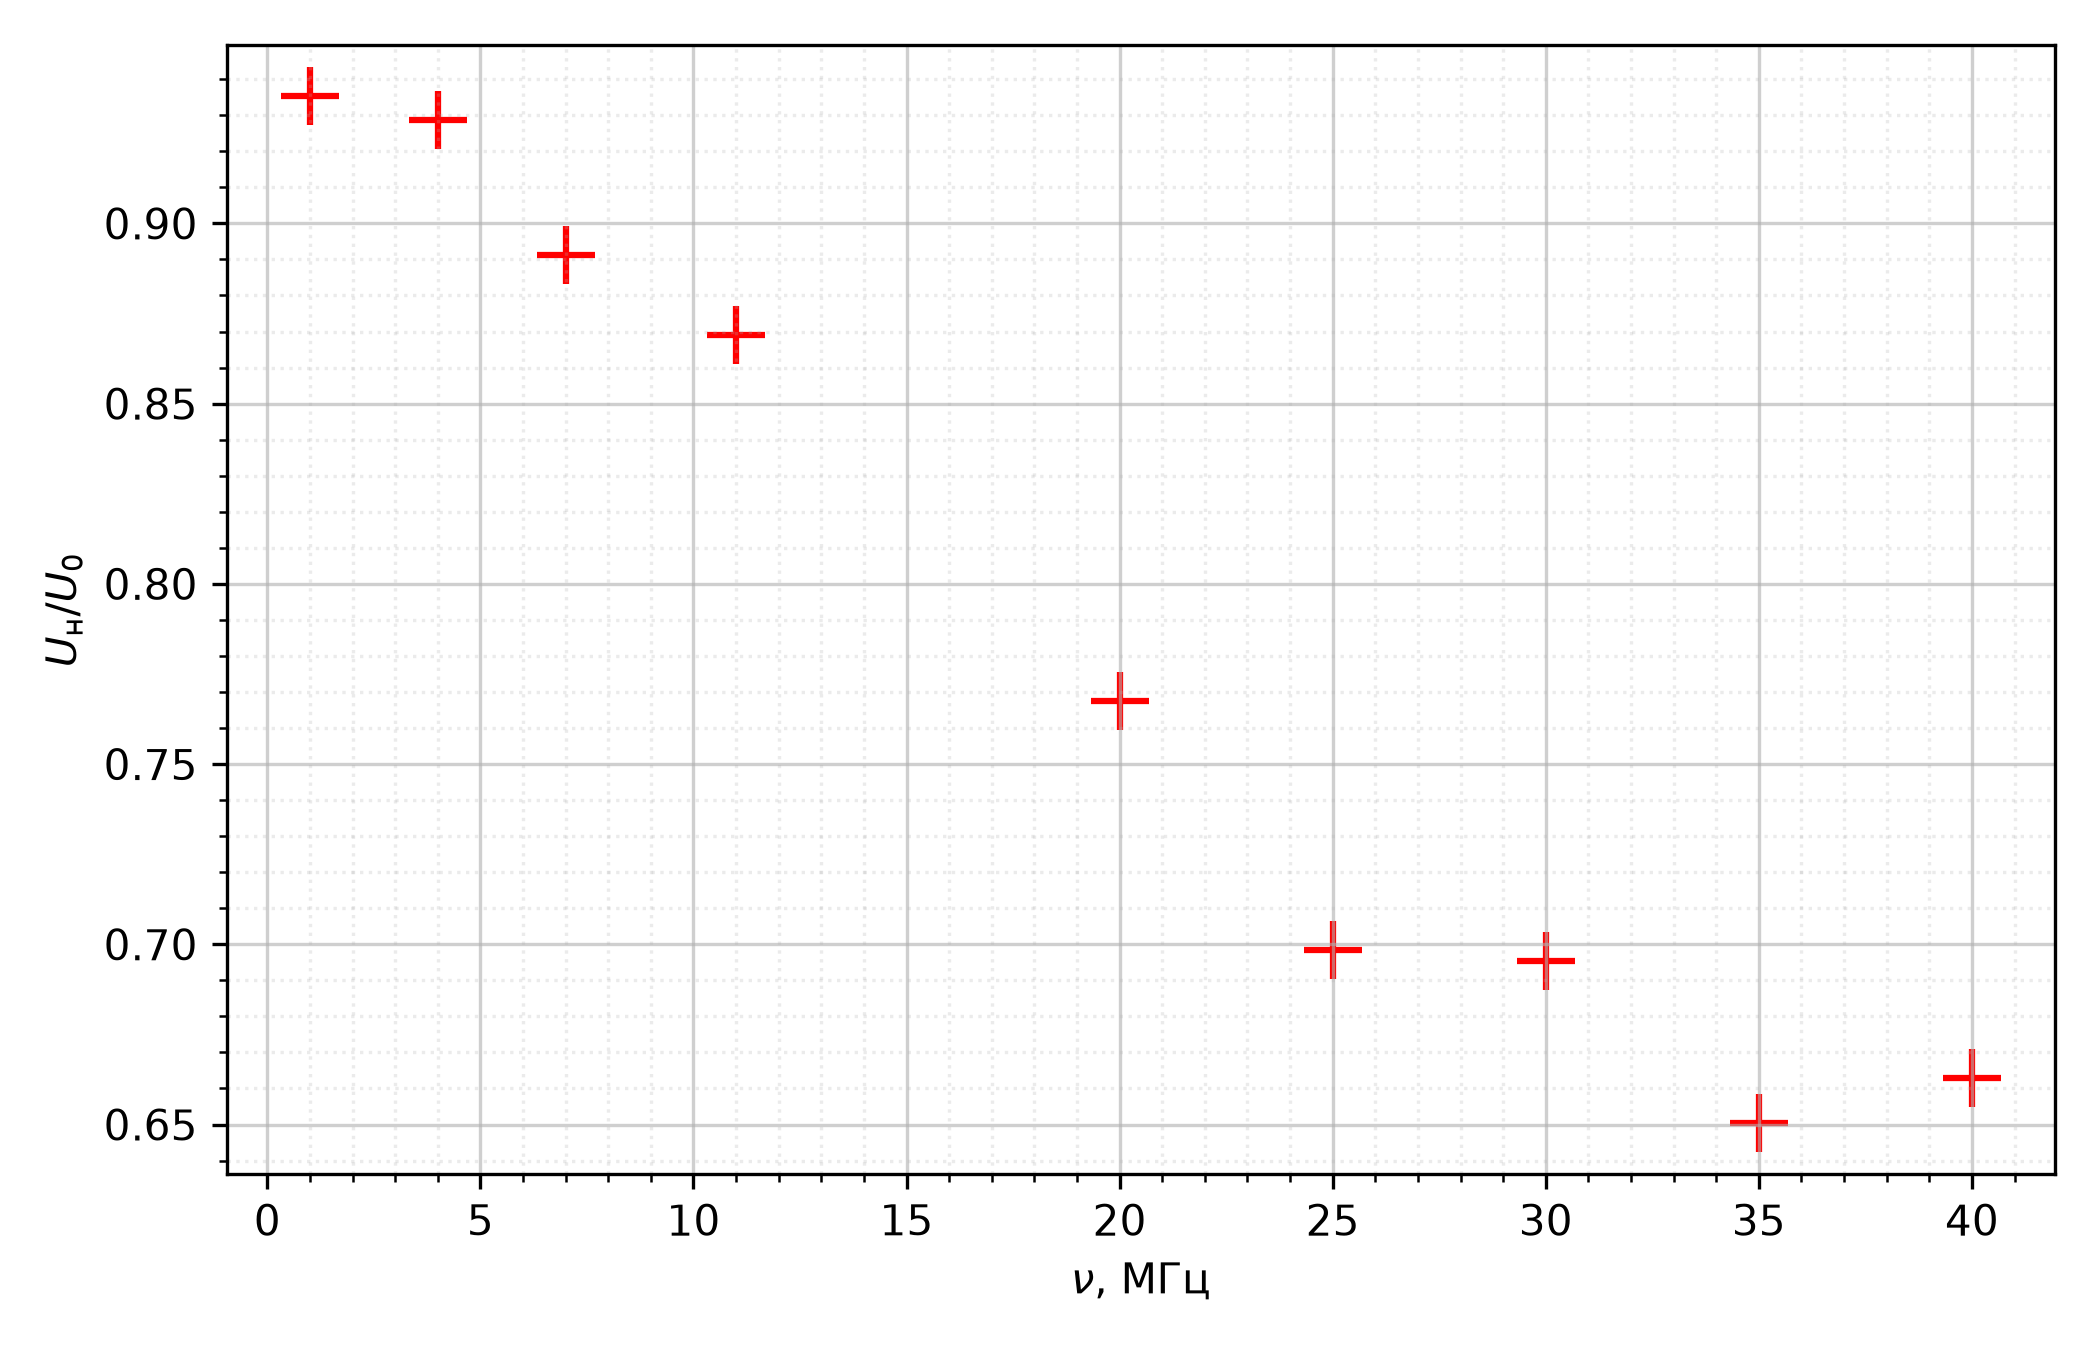
\includegraphics[width=0.85\textwidth]{figures/achx.png}
    \caption{Амплитудно-частотная характеристика длинной линии}
    \label{fig:achx}
\end{figure}

При увеличении частоты от $1$ до $40$ МГц отношение
амплитуд уменьшается от $0{,}935$ до $0{,}663$.
Таким образом, затухание сигнала возрастает с частотой.

Полный сдвиг фаз с учётом числа периодов определим
по формуле:
\begin{equation}
    \Delta\varphi = 2\pi m \pm 2\pi\nu\Delta t,
\end{equation}
где $m$ --- целое число полных периодов набега фазы.

\begin{figure}[H]
    \centering
    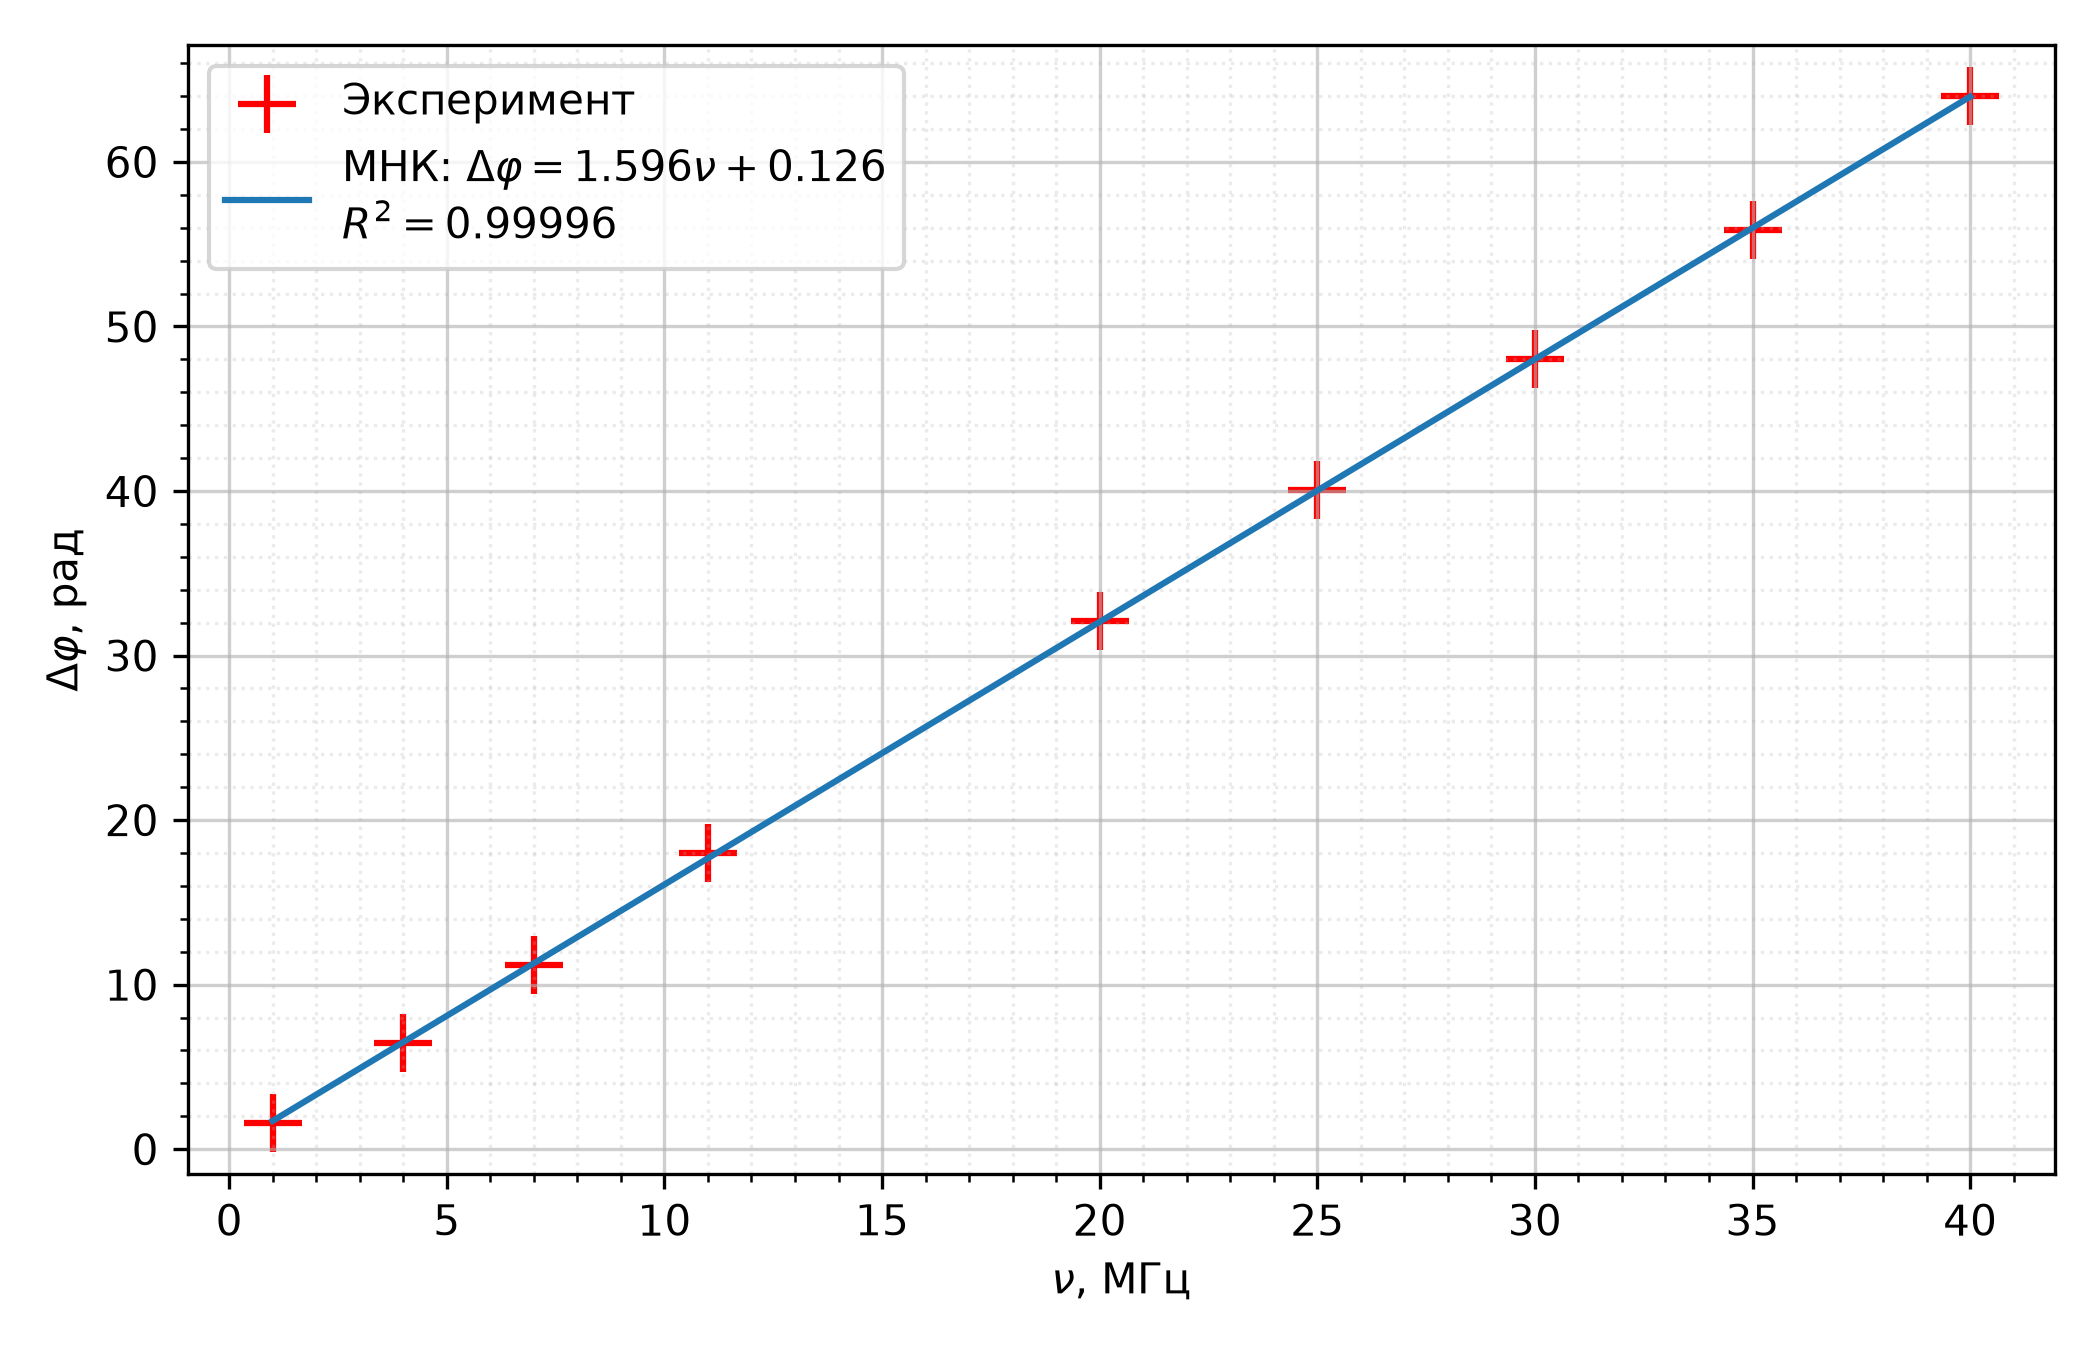
\includegraphics[width=0.85\textwidth]{figures/fchx.png}
    \caption{Фазово-частотная характеристика длинной линии}
    \label{fig:fchx}
\end{figure}

Восстановленную зависимость $\Delta\varphi(\nu)$
аппроксимируем линейной функцией:
\begin{equation}
    \Delta\varphi = a\nu + b.
\end{equation}

Методом наименьших квадратов получаем:
\[
    a = 1{,}596\ \text{рад/МГц},
    \qquad b = 0{,}126\ \text{рад}.
\]

По коэффициенту наклона определим фазовую скорость:
\begin{equation}
    V_{\text{ф}} = \frac{2\pi l}{a}\cdot 10^6
    = \frac{2\pi\cdot50{,}085}{1{,}596}\cdot10^6
    \approx 1{,}97\cdot10^8\ \text{м/с}.
\end{equation}

Полученное значение согласуется с фазовой скоростью,
найденной по резонансным частотам.
Восстановленная ФЧХ близка к линейной, что
согласуется с отсутствием заметной дисперсии.

\subsection{Определение погонных характеристик кабеля}

По экспериментальным данным вычислим коэффициент
затухания и волновое число:
\begin{equation}
    \alpha = \frac{1}{l}\ln\frac{U_0}{U_{\text{н}}},
    \qquad
    k = \frac{\Delta\varphi}{l}.
\end{equation}

В системе СИ дисперсионное соотношение имеет вид:
\begin{equation}
    k^2-\alpha^2=L_xC_x\omega^2.
\end{equation}

Построим зависимость
$y_1=k^2-\alpha^2$ от $x_1=\omega^2$.

\begin{figure}[H]
    \centering
    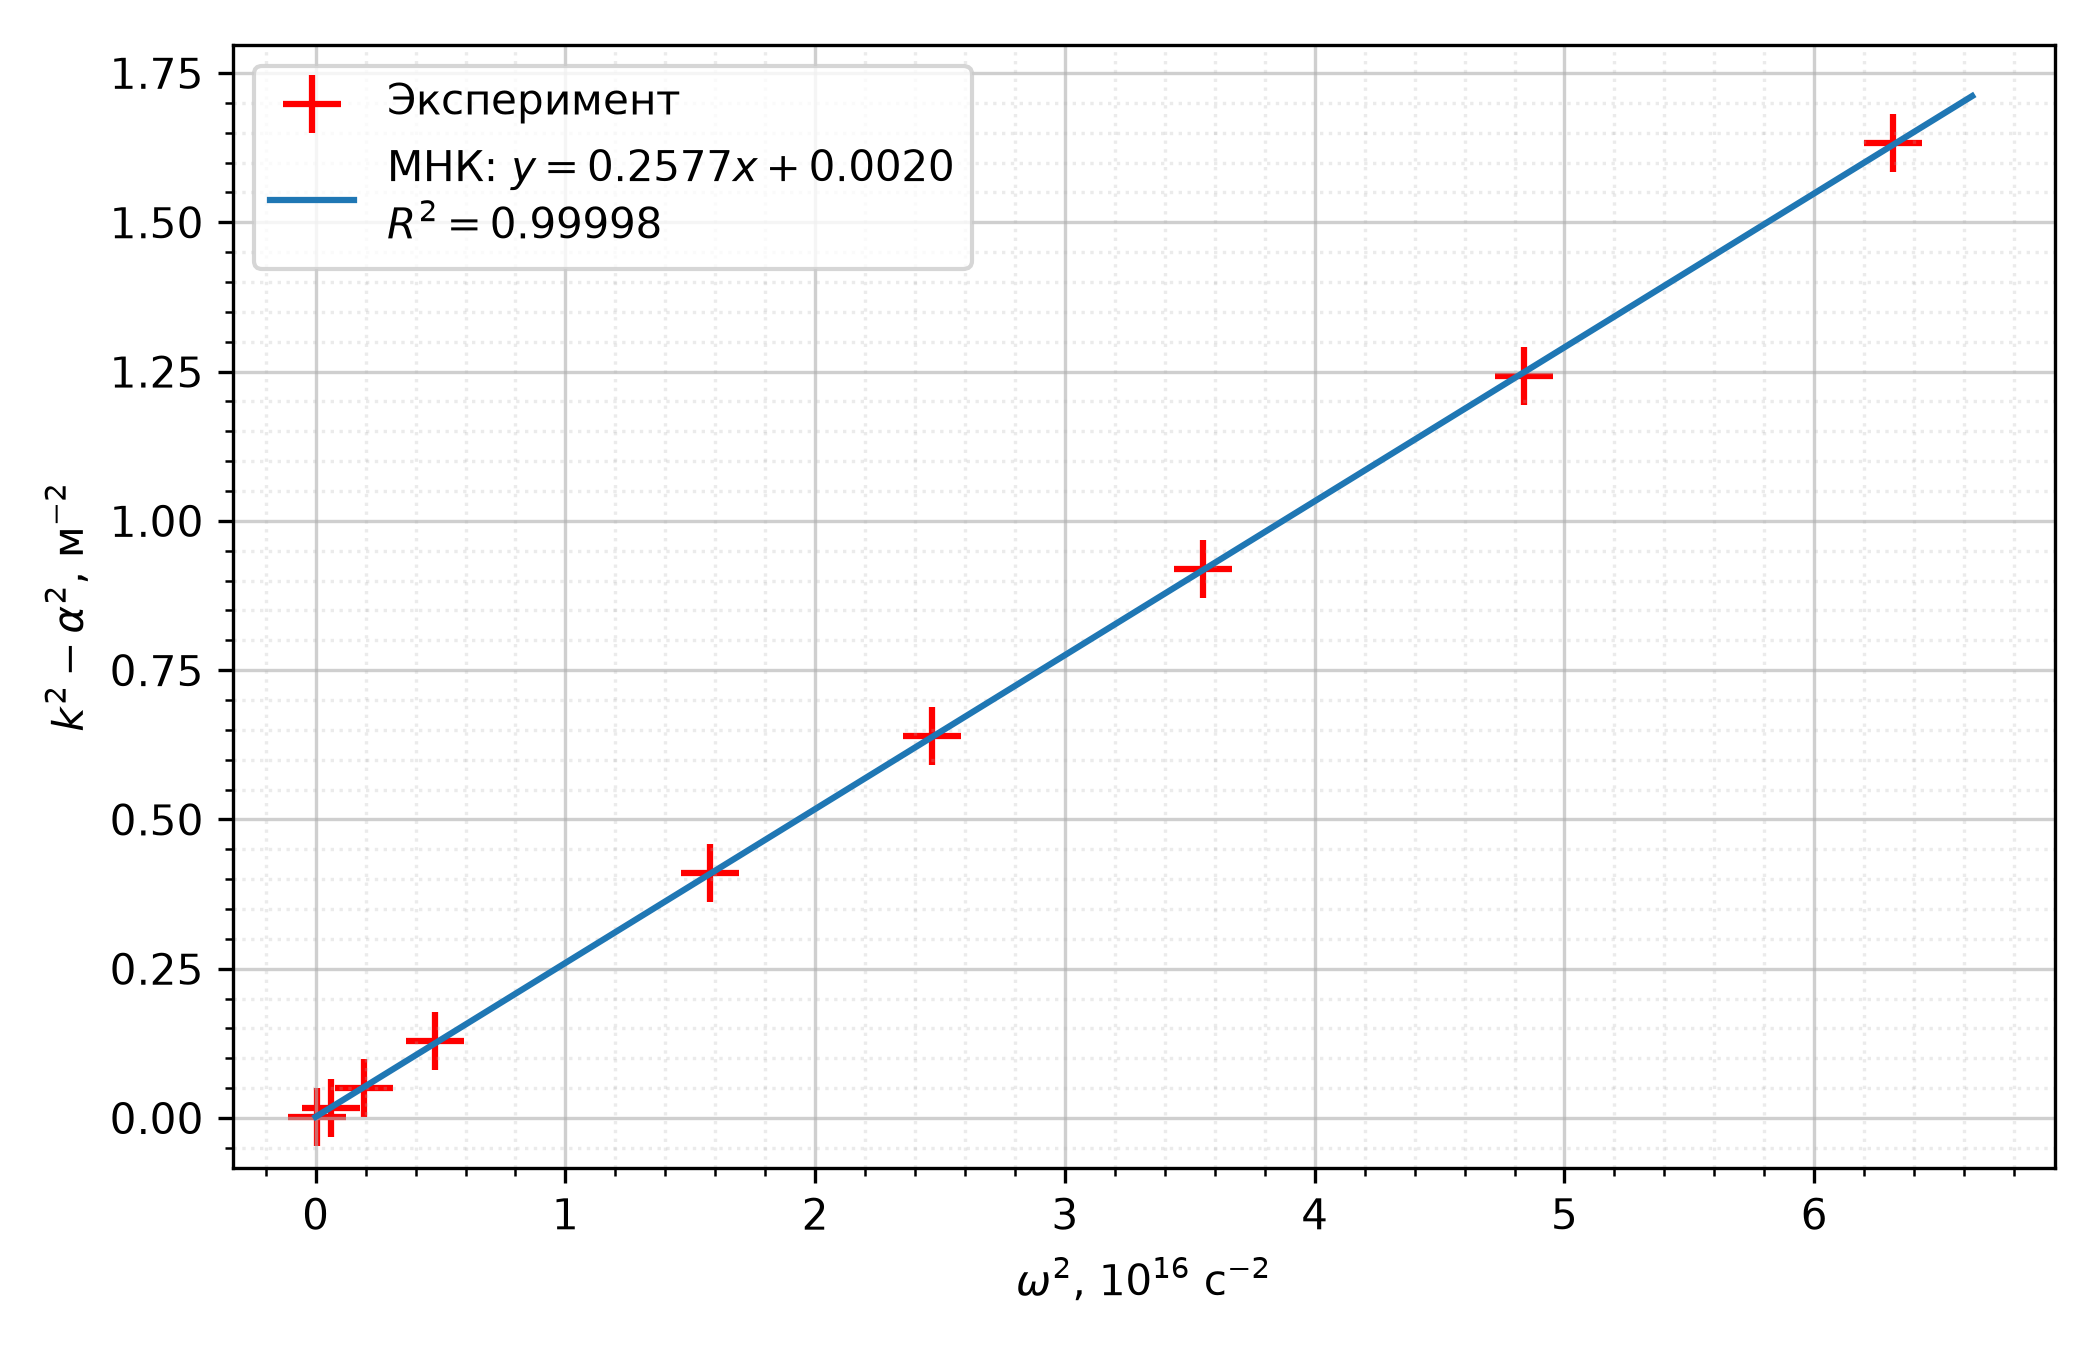
\includegraphics[width=0.85\textwidth]{figures/line_params.png}
    \caption{Зависимость разности квадратов волнового числа
    и коэффициента затухания ($k^2-\alpha^2$) от квадрата циклической частоты($\omega^2$).}
    \label{fig:line_params}
\end{figure}

Аппроксимация методом наименьших квадратов даёт:
\begin{equation}
    y_1 = 0{,}25773 x_1 + 0{,}00198,
    \qquad R^2 = 0{,}999976,
\end{equation}
где $x_1$ выражен в единицах $10^{16}$~с$^{-2}$.

Таким образом, коэффициент наклона в СИ равен:
\begin{equation}
    a = L_xC_x = 2{,}5773\cdot10^{-17}
    \ \text{с}^2/\text{м}^2.
\end{equation}

Используя волновое сопротивление $R_0=50$ Ом,
определим погонную индуктивность:
\begin{equation}
    L_x=R_0\sqrt{a}
    =50\sqrt{2{,}5773\cdot10^{-17}}
    \approx 253{,}8\ \text{нГн/м}.
\end{equation}

Аналогично найдём погонную ёмкость:
\begin{equation}
    C_x=\frac{\sqrt{a}}{R_0}
    =\frac{\sqrt{2{,}5773\cdot10^{-17}}}{50}
    \approx 101{,}5\ \text{пФ/м}.
\end{equation}

Фазовая скорость распространения сигнала:
\begin{equation}
    V_{\text{ф}}=\frac{1}{\sqrt{L_xC_x}}
    \approx 1{,}97\cdot10^8\ \text{м/с}.
\end{equation}

Полученная фазовая скорость согласуется
с оценкой по резонансным частотам
$V_{\text{ф}}\approx1{,}96\cdot10^8$ м/с.
Погонные параметры имеют физически
правдоподобные значения для коаксиального кабеля.

\subsection{Определение диэлектрической и магнитной проницаемостей}

Используя геометрические параметры коаксиального кабеля,
определим относительные диэлектрическую и магнитную
проницаемости материала между проводниками.

Отношение радиусов проводников:
\[
    \frac{r_2}{r_1}=3{,}08.
\]

В системе СИ погонные характеристики определяются
выражениями:
\begin{equation}
    L_x=\frac{\mu_0\mu_r}{2\pi}
    \ln\frac{r_2}{r_1},
    \qquad
    C_x=\frac{2\pi\varepsilon_0\varepsilon_r}
    {\ln(r_2/r_1)}.
\end{equation}

Отсюда относительная диэлектрическая проницаемость:
\begin{equation}
    \varepsilon_r=
    \frac{C_x}{2\pi\varepsilon_0}
    \ln\frac{r_2}{r_1}
    =
    \frac{101{,}5\cdot10^{-12}}
    {2\pi\cdot8{,}854\cdot10^{-12}}
    \ln(3{,}08)
    \approx 2{,}05.
\end{equation}

Относительная магнитная проницаемость:
\begin{equation}
    \mu_r=
    \frac{2\pi L_x}
    {\mu_0\ln(r_2/r_1)}
    =
    \frac{2\pi\cdot253{,}8\cdot10^{-9}}
    {4\pi\cdot10^{-7}\ln(3{,}08)}
    \approx 1{,}13.
\end{equation}

Полученная диэлектрическая проницаемость
характерна для полимерных диэлектриков.
Магнитная проницаемость отличается от
ожидаемого значения $\mu_r\approx1$ на $13\%$,
что может быть связано с погрешностями
экспериментальных измерений.

\subsection{Определение удельной проводимости. Метод А}

Согласно теории, коэффициент затухания
гармонического сигнала определяется выражением:
\begin{equation}
    \alpha(\nu)=\frac{1}{l}
    \ln\frac{U_0}{U_{\text{н}}}.
\end{equation}

С учётом скин-эффекта в системе СИ:
\begin{equation}
    \delta=\frac{1}{\sqrt{\pi\mu_0\sigma\nu}},
    \qquad
    R_x=\frac{2}{\pi d\sigma\delta}.
\end{equation}

Поскольку $\alpha=R_x/(2R_0)$, получаем:
\begin{equation}
    \alpha(\nu)=
    \frac{1}{R_0d}
    \sqrt{\frac{\mu_0}{\pi\sigma}}\sqrt{\nu}.
\end{equation}

Таким образом, зависимость $\alpha(\sqrt{\nu})$
должна быть линейной и проходить через начало координат.

\begin{figure}[H]
    \centering
    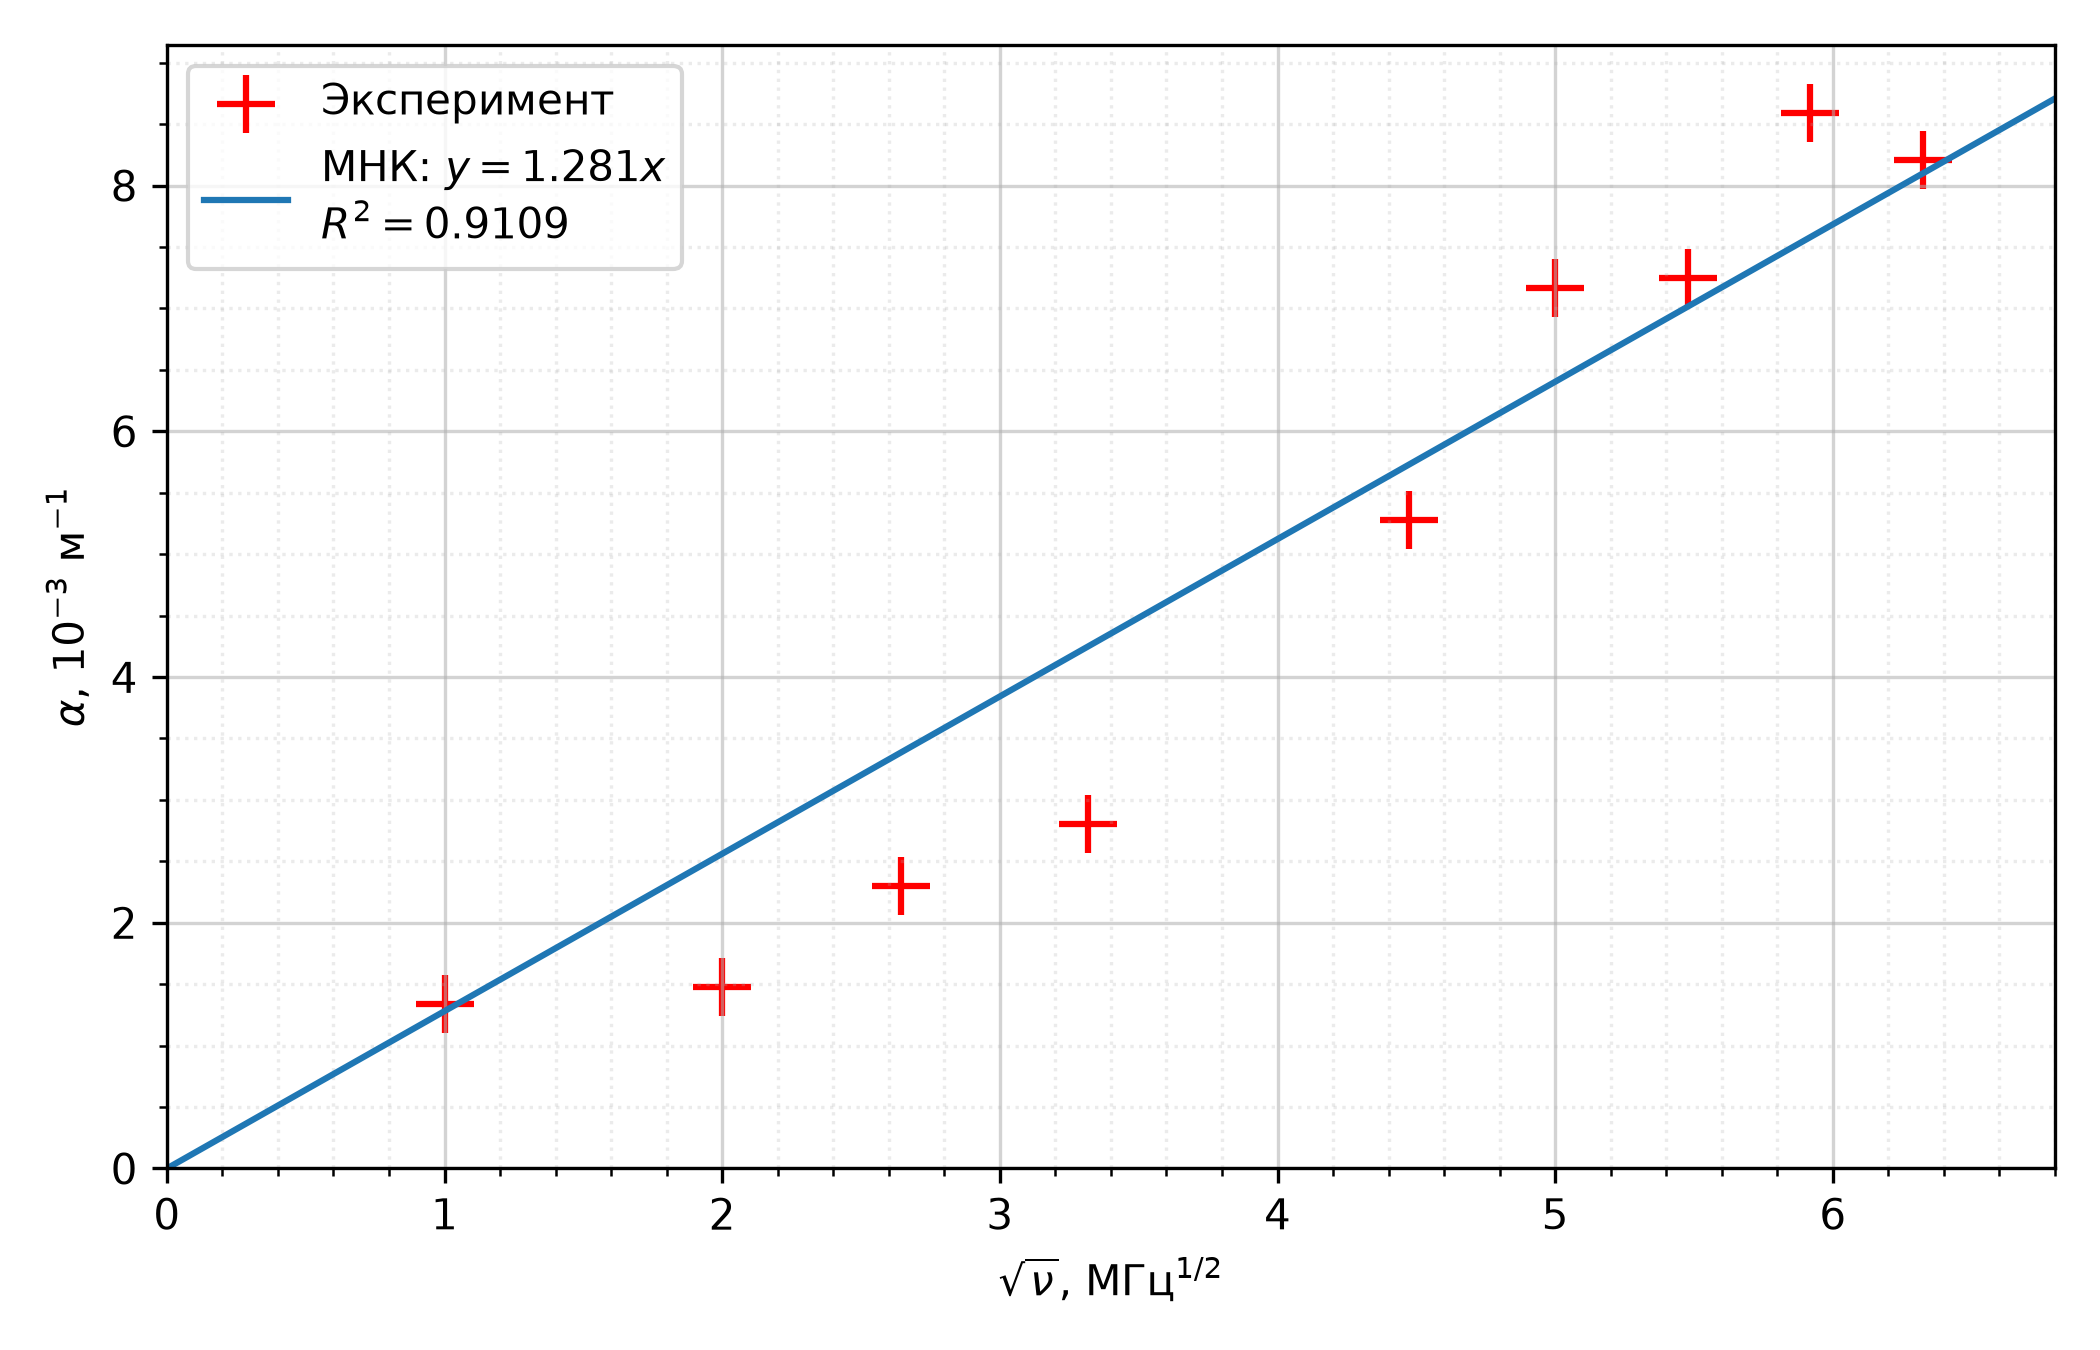
\includegraphics[width=0.85\textwidth]{figures/metod_A.png}
    \caption{Зависимость коэффициента затухания ($\alpha$)
от квадратного корня частоты ($\sqrt{\nu}$).}
    \label{fig:metod_A}
\end{figure}

Аппроксимацией методом наименьших квадратов
с нулевым свободным членом получаем:
\begin{equation}
    a=(1{,}281\pm0{,}068)\cdot10^{-6}
    \ \frac{1}{\text{м}\sqrt{\text{Гц}}},
    \qquad R^2=0{,}9109.
\end{equation}

Из коэффициента наклона выразим удельную проводимость:
\begin{equation}
    \sigma=\frac{\mu_0}{\pi R_0^2d^2a^2}.
\end{equation}

Подставляя экспериментальные значения:
\begin{equation}
    \sigma=
    \frac{4\pi\cdot10^{-7}}
    {\pi(50\cdot1{,}37\cdot10^{-3}
    \cdot1{,}281\cdot10^{-6})^2}
    \approx5{,}20\cdot10^7\ \text{См/м}.
\end{equation}

Сравним полученное значение с табличной
проводимостью меди $\sigma_{\text{Cu}}=5{,}8\cdot10^7$
См/м:
\begin{equation}
    \delta_\sigma=
    \frac{|\sigma-\sigma_{\text{Cu}}|}
    {\sigma_{\text{Cu}}}\cdot100\%
    \approx10{,}4\%.
\end{equation}

Экспериментальные данные в целом согласуются
с зависимостью $\alpha\propto\sqrt{\nu}$.
Полученная проводимость отличается от табличного
значения для меди на $10{,}4\%$.
Разброс экспериментальных точек относительно
аппроксимирующей прямой может быть связан
с погрешностями измерений и дополнительными
потерями в кабеле.

\subsection{Определение удельной проводимости. Метод Б}

Из телеграфных уравнений получаем соотношение:
\begin{equation}
    2\alpha k = \omega R_x C_x.
\end{equation}

С учётом скин-эффекта в системе СИ:
\begin{equation}
    R_x = \frac{2}{d}
    \sqrt{\frac{\mu_0\nu}{\pi\sigma}}.
\end{equation}

Следовательно,
\begin{equation}
    \alpha k =
    \frac{2C_x}{d}
    \sqrt{\frac{\pi\mu_0}{\sigma}}\nu^{3/2}.
\end{equation}

Построим зависимость $y_3=\alpha k$ от
$x_3=\nu^{3/2}$.

\begin{figure}[H]
    \centering
    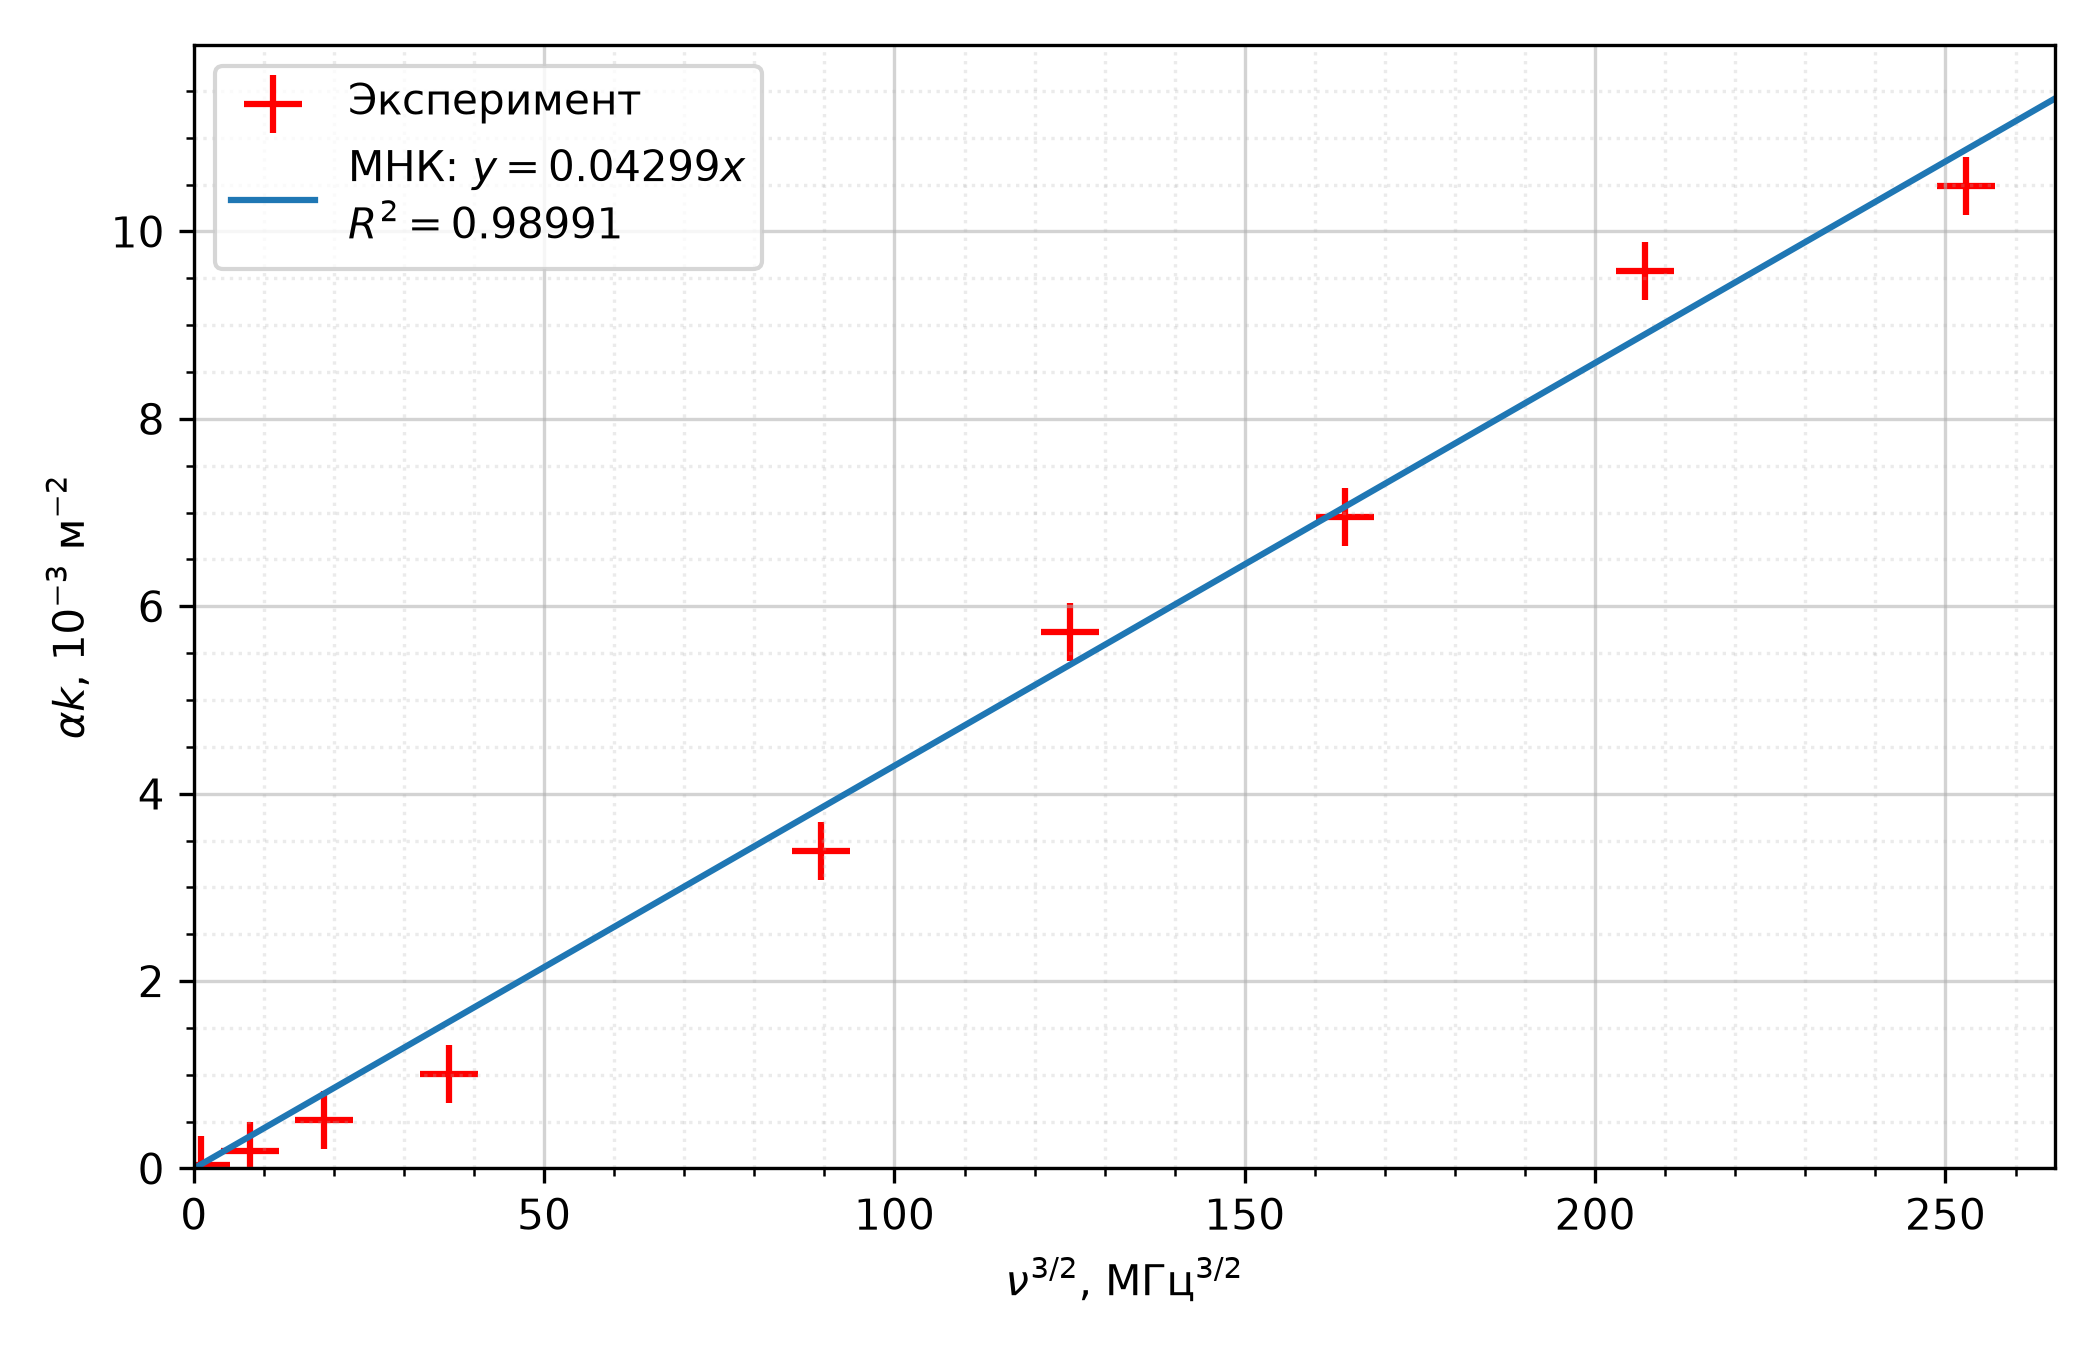
\includegraphics[width=0.85\textwidth]{figures/metod_B.png}
    \caption{Зависимость произведения коэффициента затухания
и волнового числа ($\alpha k$) от частоты в степени
$3/2$ ($\nu^{3/2}$).}
    \label{fig:metod_B}
\end{figure}

Аппроксимация методом наименьших квадратов
через начало координат даёт:
\begin{equation}
    y_3 = 0{,}04299 x_3,
    \qquad R^2 = 0{,}98991,
\end{equation}
где $y_3$ выражен в единицах
$10^{-3}$ м$^{-2}$, а частота в МГц.

Таким образом, коэффициент наклона в СИ:
\begin{equation}
    a = 4{,}299\cdot10^{-14}
    \ \frac{1}{\text{м}^2\cdot\text{Гц}^{3/2}}.
\end{equation}

Выразим удельную проводимость:
\begin{equation}
    \sigma=\frac{4\pi\mu_0 C_x^2}{d^2a^2}.
\end{equation}

Подставляя экспериментальные значения:
\begin{equation}
    \sigma =
    \frac{
        4\pi\cdot(4\pi\cdot10^{-7})
        \cdot(101{,}5\cdot10^{-12})^2
    }{
        (1{,}37\cdot10^{-3})^2
        \cdot(4{,}299\cdot10^{-14})^2
    }
    \approx 4{,}69\cdot10^7\ \text{См/м}.
\end{equation}

Сравним результат с табличной проводимостью меди:
\begin{equation}
    \delta_\sigma =
    \frac{|\sigma-\sigma_{\mathrm{Cu}}|}
    {\sigma_{\mathrm{Cu}}}\cdot100\%
    \approx 19{,}1\%.
\end{equation}

\subsection{Сравнение результатов методов А и Б}

Методом А получено:
\[
    \sigma_A=5{,}20\cdot10^7\ \text{См/м}.
\]

Методом Б получено:
\[
    \sigma_B=4{,}69\cdot10^7\ \text{См/м}.
\]

Относительное расхождение результатов:
\begin{equation}
    \delta_{AB}=
    \frac{|\sigma_A-\sigma_B|}{\sigma_A}
    \cdot100\%\approx9{,}75\%.
\end{equation}

Оба метода дают проводимость одного порядка
с табличным значением для меди.
Метод А обеспечивает меньшее отклонение
от табличного значения (10,4\% против 19,1\%).

Полученные зависимости качественно
согласуются с моделью скин-эффекта.

\newpage

% ==================== МОДЕЛЬ ====================
\section{Модель длинной линии}

\subsection{Предельная частота и согласованная нагрузка}
В модели используются ячейки с индуктивностью $L=1{,}5\,\text{мГн}$
и ёмкостью $C=47\,\text{нФ}$ (на концах линии --- $C/2$).
Для модели используем СИ.

\begin{equation}
    \nu_0=\frac{1}{\pi\sqrt{LC}},
    \qquad
    R_0=\sqrt{\frac{L}{C}}.
\end{equation}

Расчёт: $\nu_0=37,9$~кГц, $R_0=178,6$~Ом.

\subsection{Фазовый сдвиг между соседними ячейками}
Для $8$--$10$ частот измерен сдвиг фаз между соседними ячейками.

\begin{table}[H]
    \centering
    \caption{Зависимость сдвига фаз от частоты}
    \begin{tabular}{c|c}
        \toprule
        $\nu$, кГц & $\Delta\varphi$, град\\
        \midrule
        1 & 6,34 \\
        3 & 16,77 \\
        6 & 32,21 \\
        10 & 50,83 \\
        15 & 78,44 \\
        20 & 101,2 \\
        23 & 118,6 \\
        24 & 122,9 \\
        27 & 136,0 \\
        30 & 154,8 \\
        33 & 166,0 \\
        \bottomrule
    \end{tabular}
\end{table}

Для дискретной модели длинной линии расчётная
зависимость фазового сдвига между соседними
ячейками от частоты имеет вид:
\begin{equation}
    \Delta\varphi_{\text{теор}} =
    2\arcsin\left(\frac{\nu}{\nu_0}\right),
    \qquad \nu < \nu_0.
\end{equation}

По экспериментальным данным построим зависимость
$\Delta\varphi(\nu)$ и сравним её с теоретической.

\begin{figure}[H]
    \centering
    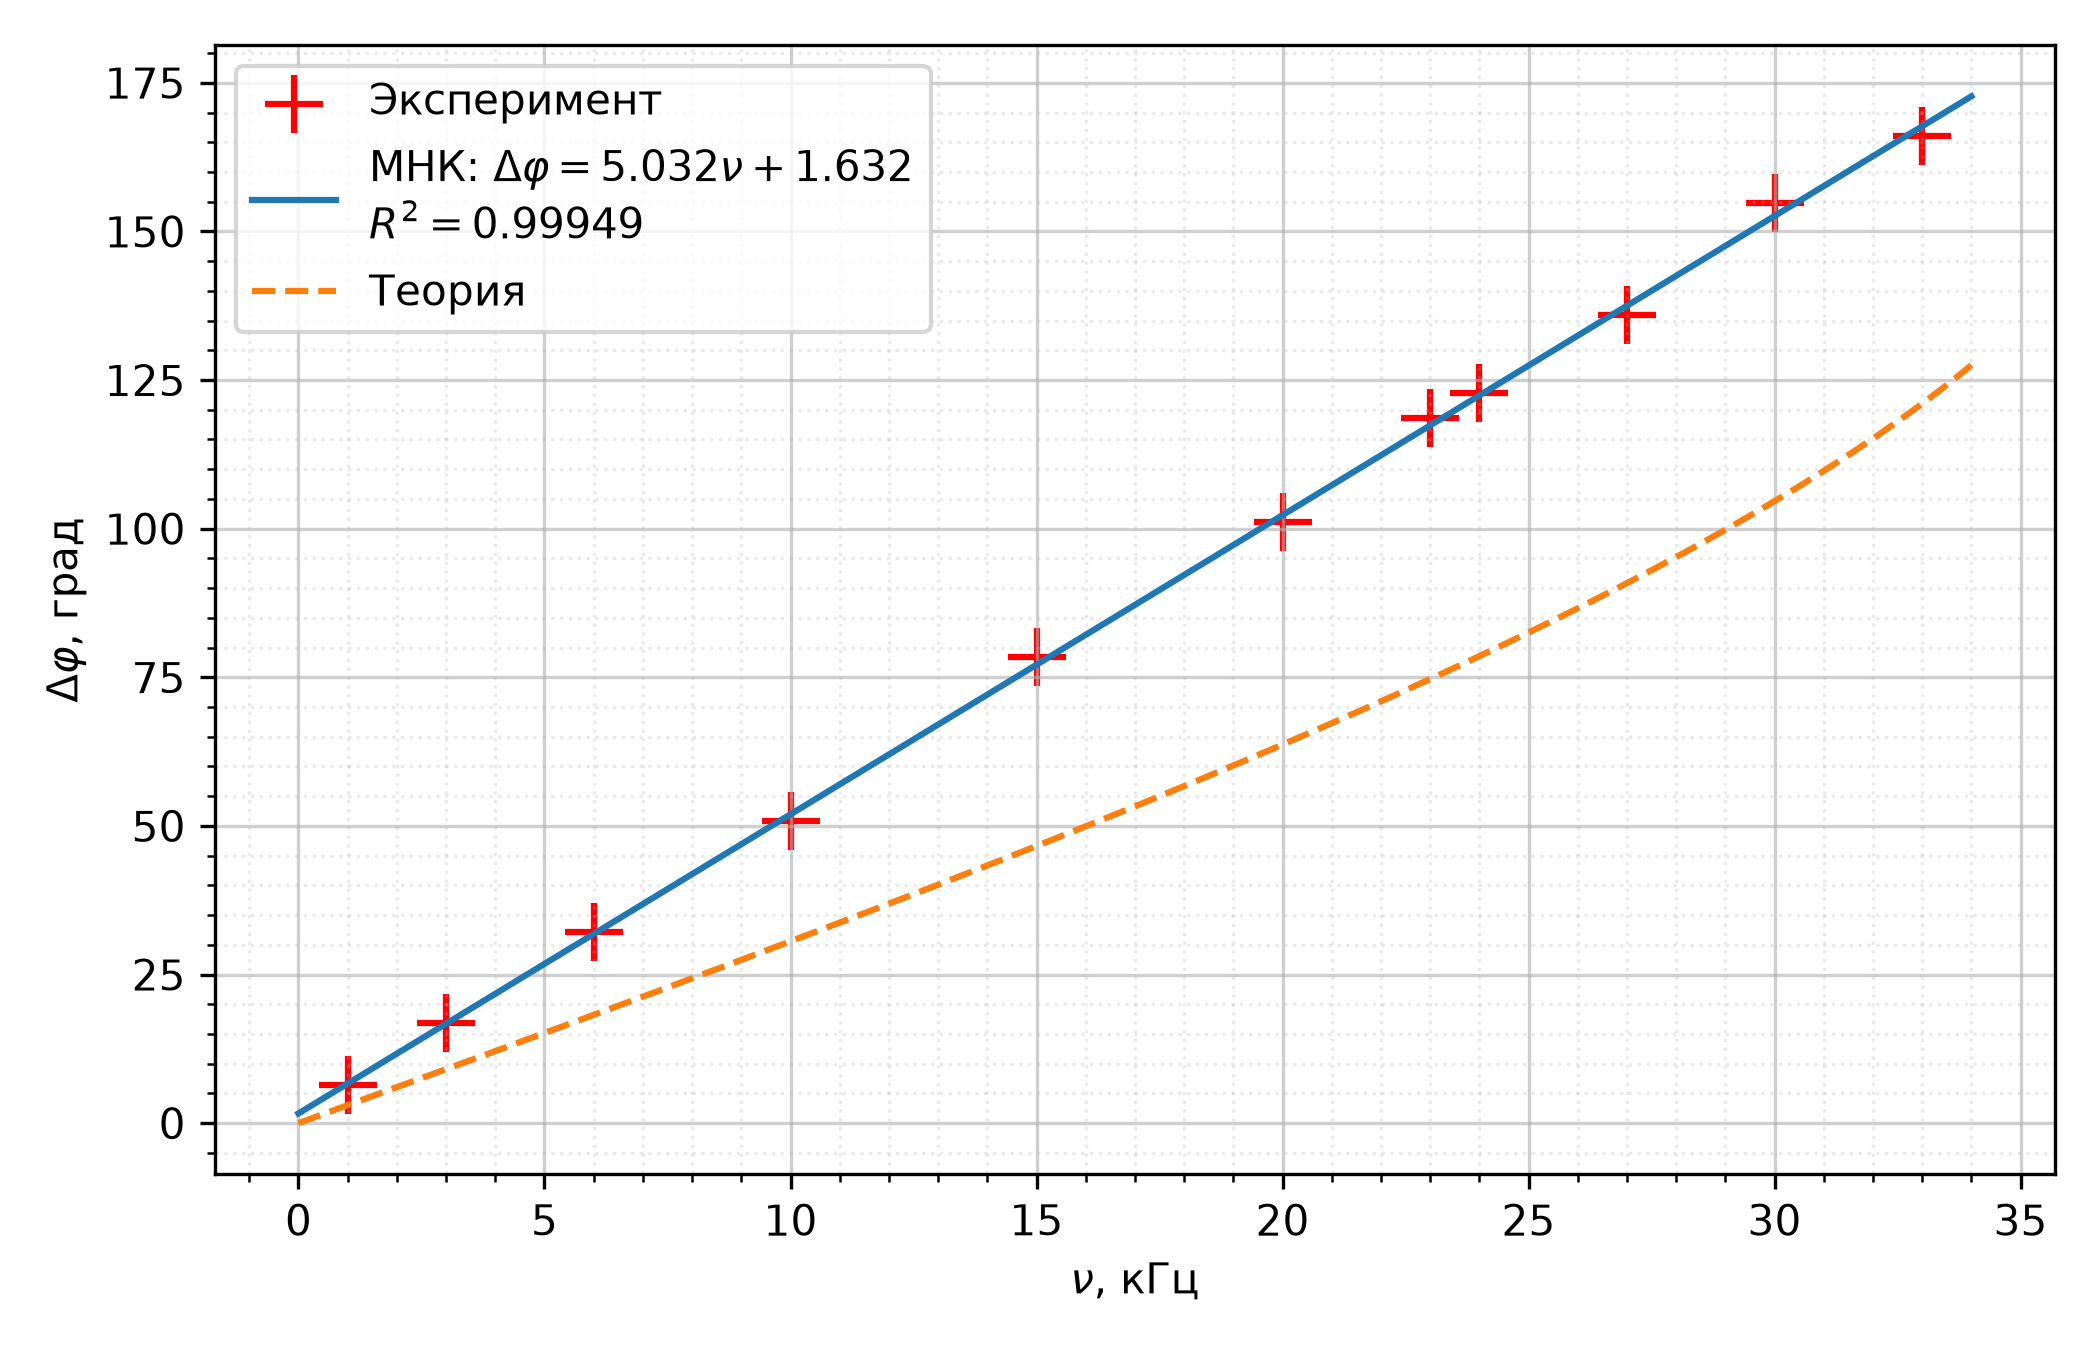
\includegraphics[width=0.85\textwidth]{figures/model_phase.png}
    \caption{Зависимость фазового сдвига между соседними ячейками
($\Delta\varphi$) от частоты ($\nu$).}
    \label{fig:model_phase}
\end{figure}

Аппроксимация экспериментальных данных методом
наименьших квадратов даёт:
\begin{equation}
    \Delta\varphi = 5{,}032\nu + 1{,}632,
    \qquad R^2 = 0{,}99949,
\end{equation}
где $\nu$ выражена в кГц, а $\Delta\varphi$ ---
в градусах.

Экспериментальная зависимость близка к линейной,
однако наблюдается заметное расхождение
с теоретической кривой.

При частоте $\nu=33$ кГц:
\begin{equation}
    \Delta\varphi_{\text{теор}}\approx121{,}0^\circ,
    \qquad
    \Delta\varphi_{\text{эксп}}=166{,}0^\circ.
\end{equation}

Относительное расхождение составляет:
\begin{equation}
    \delta =
    \frac{166{,}0-121{,}0}{121{,}0}
    \cdot100\%
    \approx37{,}2\%.
\end{equation}

Таким образом, эксперимент подтверждает
увеличение фазового сдвига с частотой,
однако количественное согласие с расчётной
зависимостью неудовлетворительное.
Причиной могут быть отклонения параметров
элементов от номинальных значений
или систематические ошибки измерения фазы.

\subsection{Распределение амплитуды вдоль линии}

Для трёх резонансных частот $10$, $19{,}2$ и $26{,}6$ кГц
измерены амплитуды напряжения на ячейках с номерами от $4$ до $10$.

\begin{table}[H]
    \centering
    \caption{Распределение амплитуды напряжения вдоль линии}
    \label{tab:model_amplitudes}
    \small
    \setlength{\tabcolsep}{10pt}
    \renewcommand{\arraystretch}{1.15}
    \begin{tabular}{cccc}
        \toprule
        Номер ячейки & $U(10\,\text{кГц})$, В
        & $U(19{,}2\,\text{кГц})$, В
        & $U(26{,}6\,\text{кГц})$, В \\
        \midrule
        4  & 32,7 & 43,0 & 51,5 \\
        5  & 66,5 & 64,5 & 45,6 \\
        6  & 39,0 & 45,0 & 37,5 \\
        7  & 28,0 & 43,3 & 35,0 \\
        8  & 26,0 & 42,5 & 32,5 \\
        9  & 33,0 & 36,0 & 30,5 \\
        10 & 36,0 & 38,0 & 29,0 \\
        \bottomrule
    \end{tabular}
\end{table}

По данным таблицы~\ref{tab:model_amplitudes} построены
распределения амплитуды напряжения по номеру ячейки.

\begin{figure}[H]
    \centering
    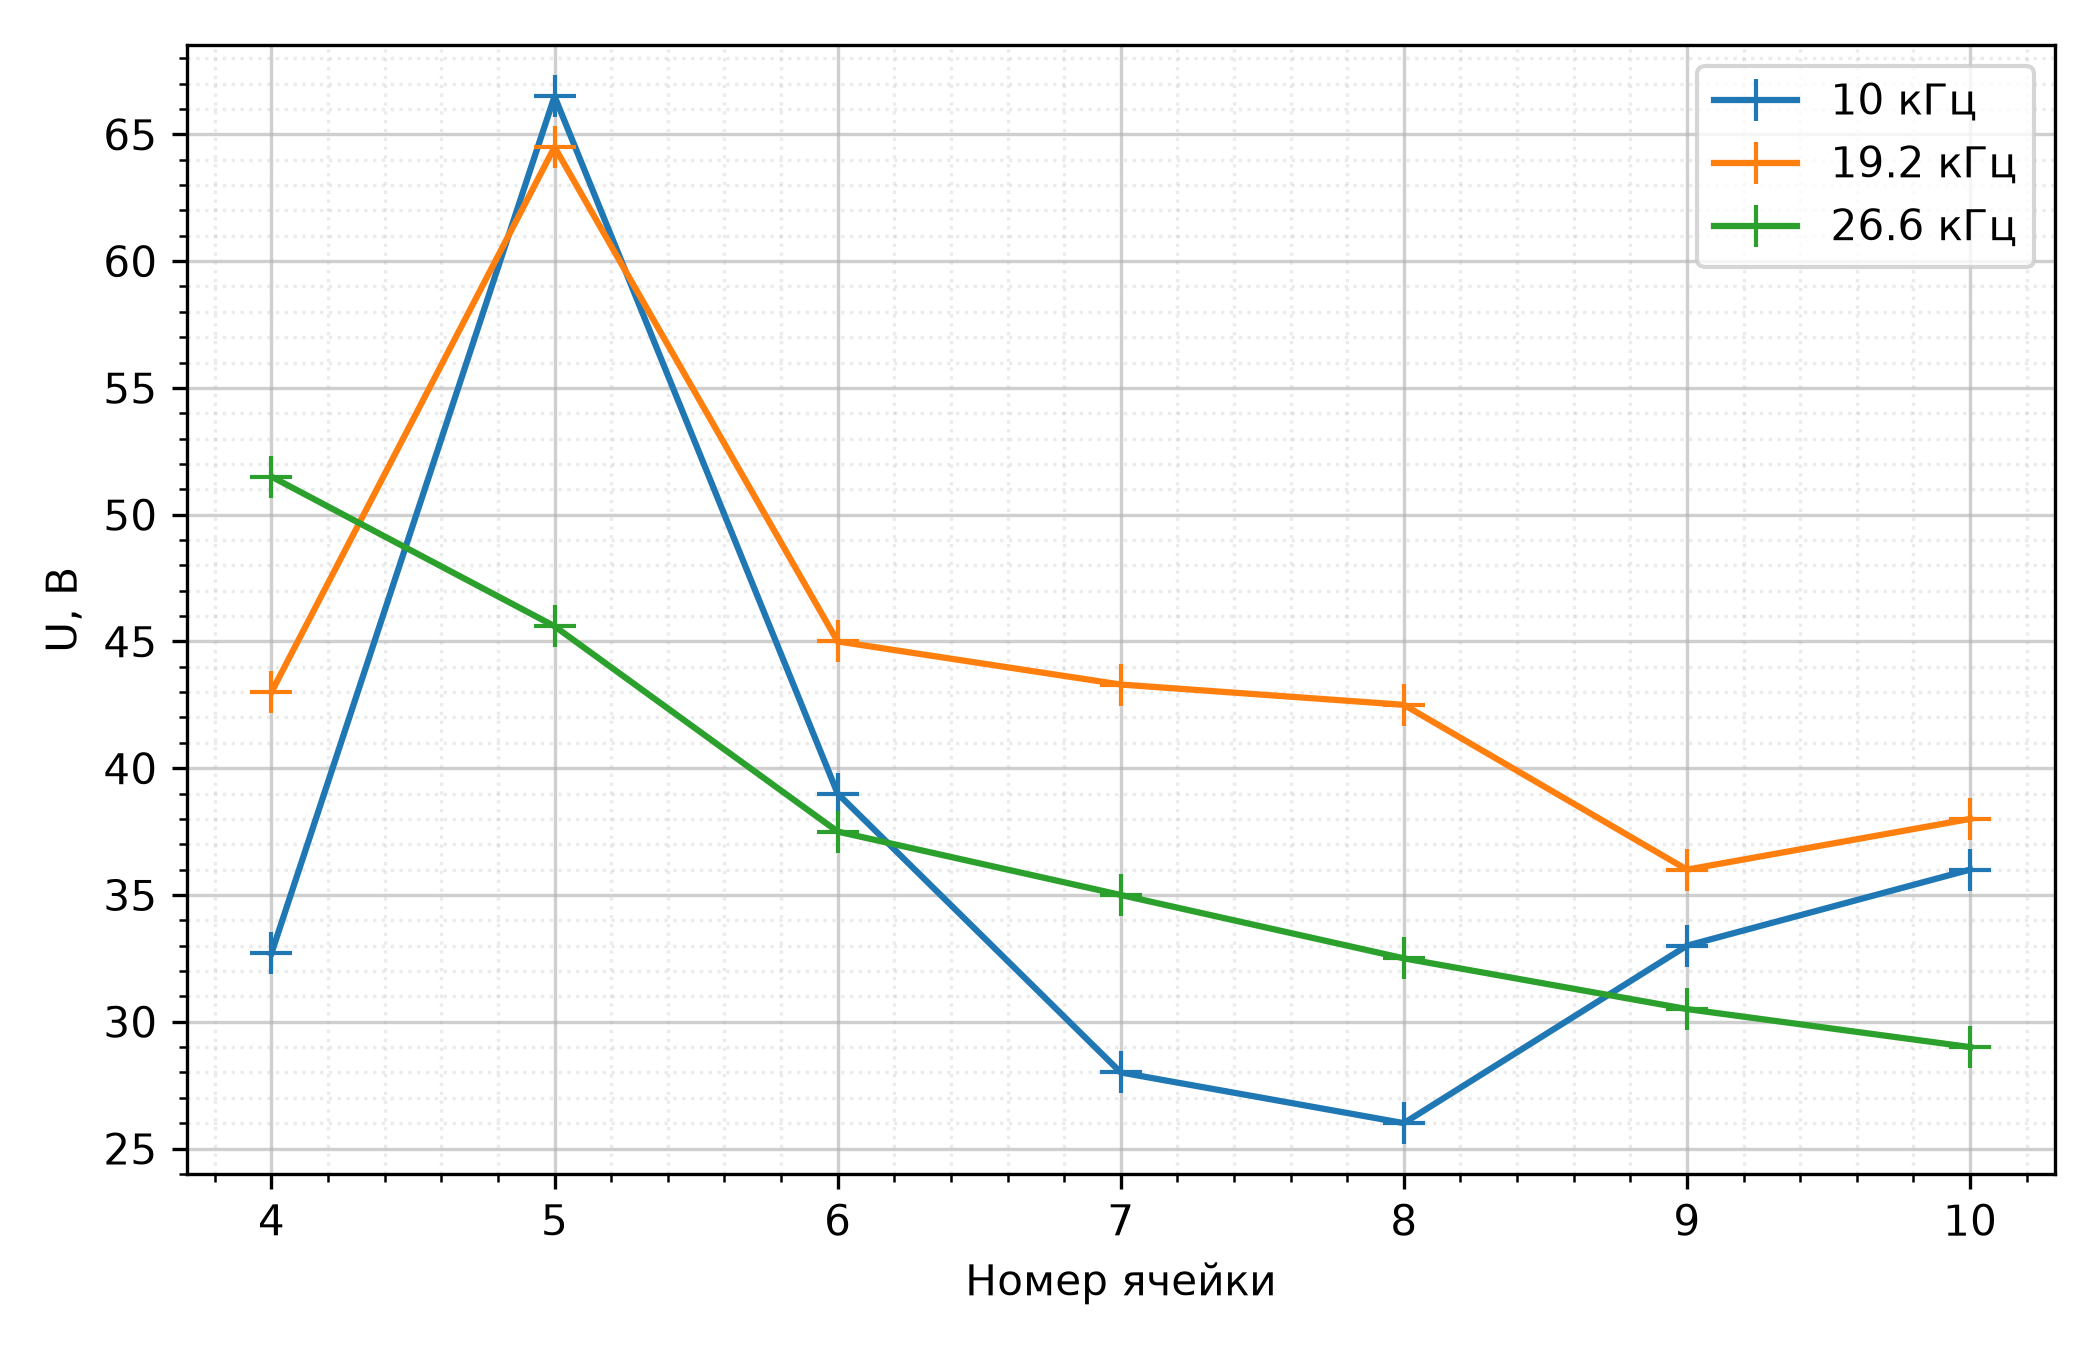
\includegraphics[width=0.85\textwidth]{figures/model_amplitudes.png}
    \caption{Распределение амплитуды напряжения вдоль линии
    при трёх резонансных частотах}
    \label{fig:model_amplitudes}
\end{figure}

При частотах $10$ и $19{,}2$ кГц максимумы напряжения
наблюдаются на ячейке №~5 и составляют соответственно
$66{,}5$ и $64{,}5$ В, а минимумы --- $26{,}0$ В
(ячейка №~8) и $36{,}0$ В (ячейка №~9).
При $26{,}6$ кГц амплитуда убывает от $51{,}5$
до $29{,}0$ В, то есть на $43{,}7\%$.


% \begin{figure}[H]
%     \centering
%     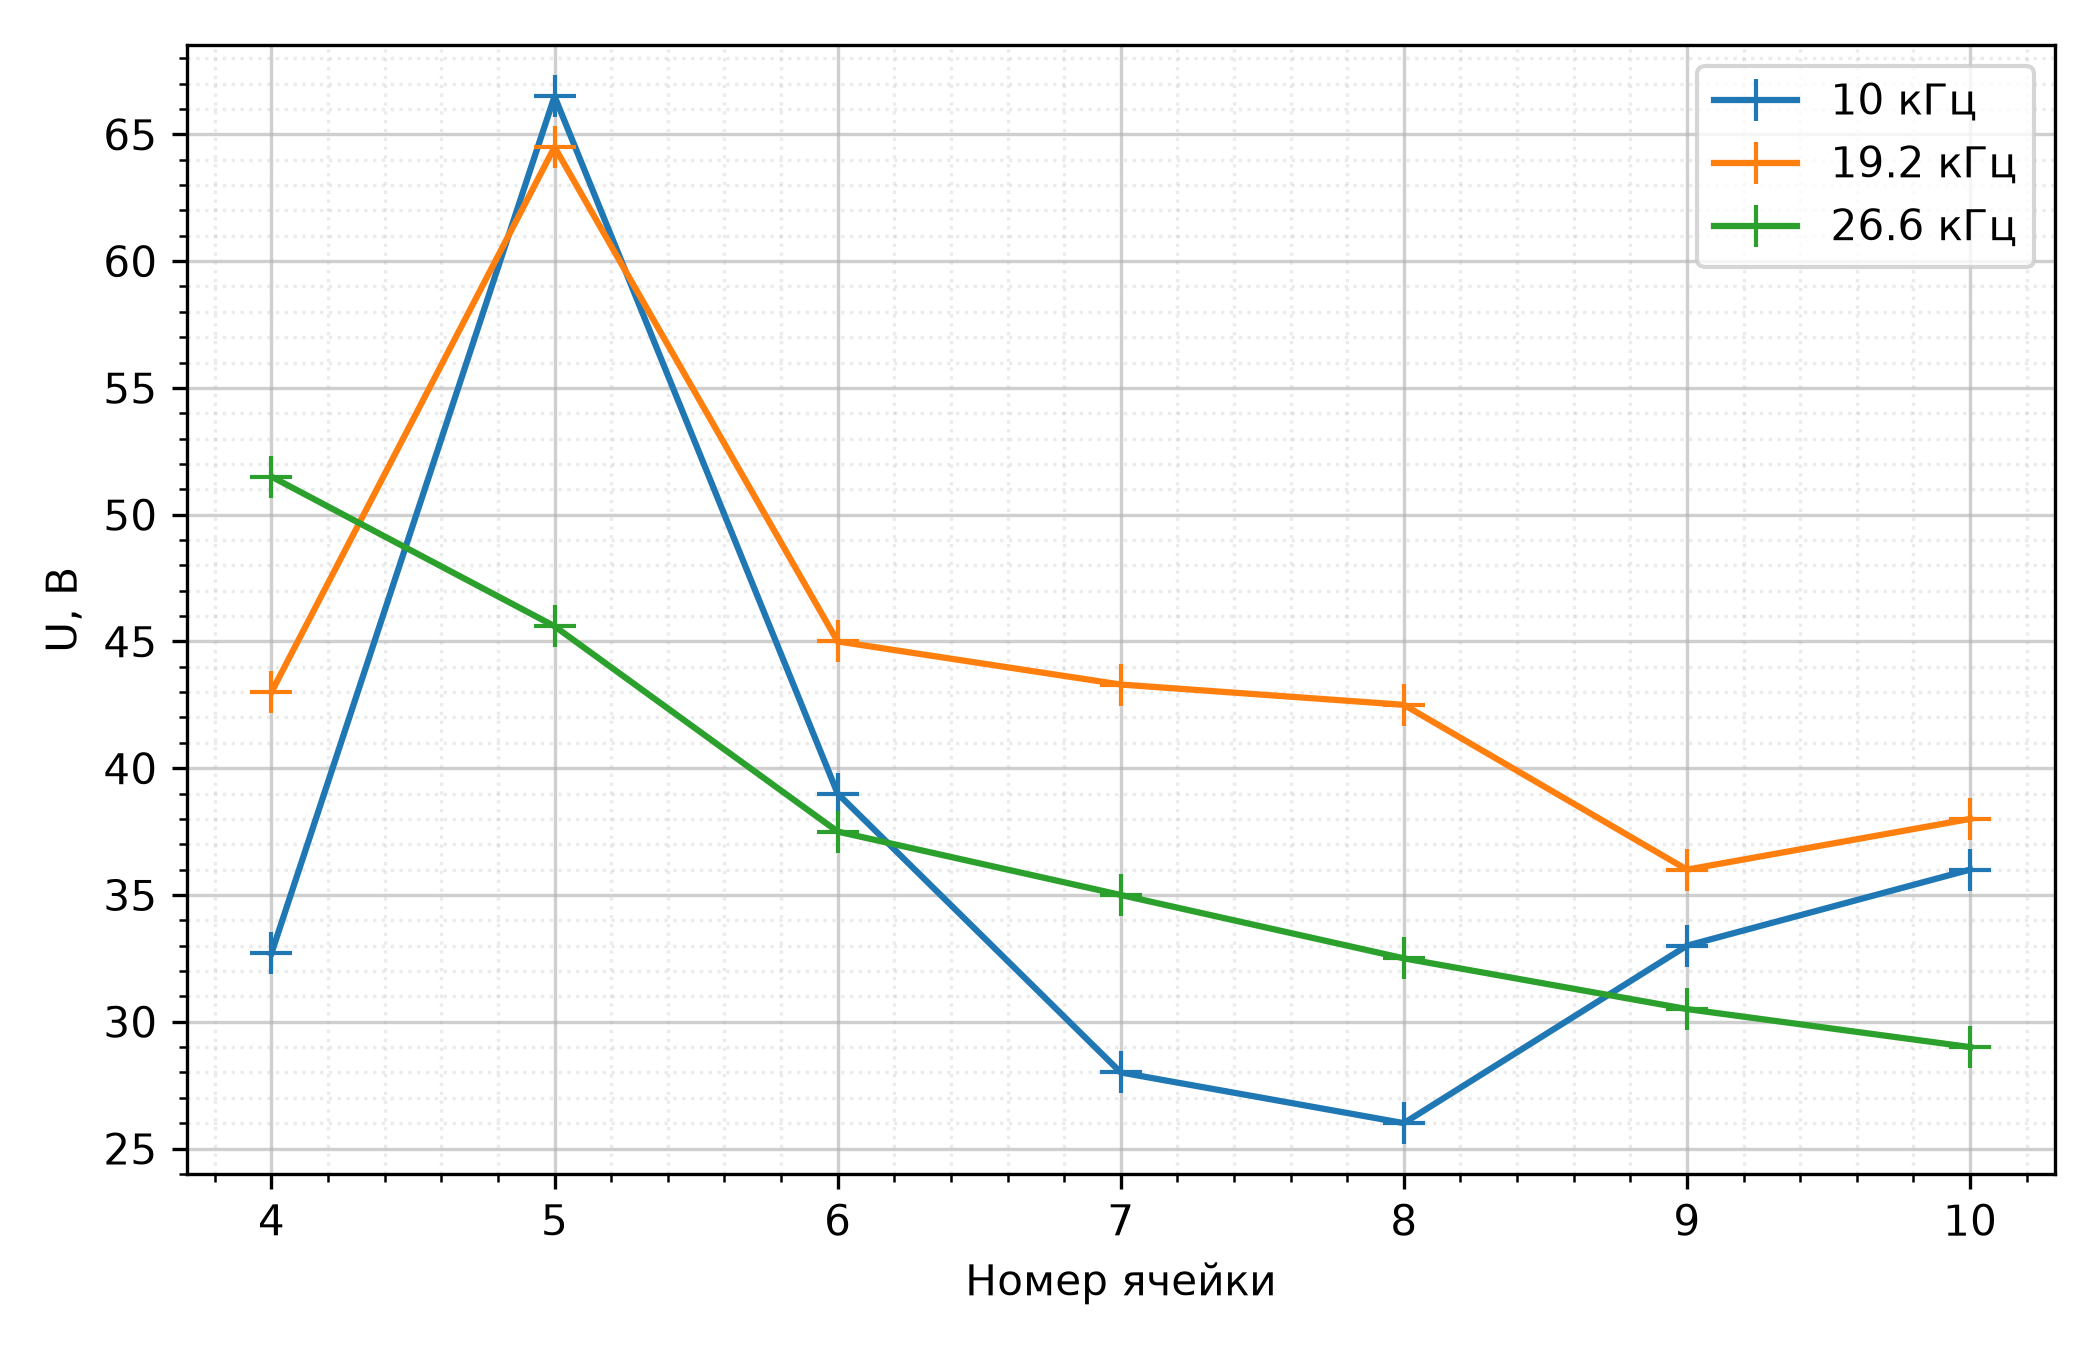
\includegraphics[width=0.85\textwidth]{figures/model_amplitudes.png}
%     \caption{Распределение амплитуды напряжения вдоль модели линии}
%     \label{fig:model_amplitudes}
% \end{figure}

% Необязательный пункт методички:
% \subsection{Резонансные кривые и добротность}
% \begin{equation}
%     Q=\frac{\nu_{\text{рез}}}{\Delta\nu}.
% \end{equation}
% \begin{figure}[H]
%     \centering
%     \includegraphics[width=0.85\textwidth]{figures/model_resonance.png}
%     \caption{Резонансные кривые модели длинной линии}
%     \label{fig:model_resonance}
% \end{figure}

\newpage

% ==================== ВЫВОД ====================
\section*{Вывод}

В ходе работы были получены следующие результаты:

Для коаксиальной длинной линии:

\begin{itemize}
    \item Фазовая скорость:
    $V_{\text{ф}} \approx 1{,}96\cdot10^8$ м/с.

    \item Групповая скорость:
    $V_{\text{гр}} \approx 1{,}95\cdot10^8$ м/с.

    \item Погонная индуктивность:
    $L_x = 253{,}8$ нГн/м.

    \item Погонная ёмкость:
    $C_x = 101{,}5$ пФ/м.

    \item Диэлектрическая проницаемость:
    $\varepsilon_r = 2{,}05$.

    \item Магнитная проницаемость:
    $\mu_r = 1{,}13$.

    \item Удельная проводимость методом А:
    $\sigma_A = 5{,}20\cdot10^7$ См/м.

    \item Удельная проводимость методом Б:
    $\sigma_B = 4{,}69\cdot10^7$ См/м.
\end{itemize}

Для дискретной модели длинной линии:

\begin{itemize}
    \item Предельная частота:
    $\nu_0 = 37{,}9$ кГц.

    \item Согласованное сопротивление:
    $R_0 = 178{,}6$ Ом.

    \item Максимальная амплитуда при $10$ кГц:
    $U_{\max} = 66{,}5$ В (ячейка №~5).

    \item Максимальная амплитуда при $19{,}2$ кГц:
    $U_{\max} = 64{,}5$ В (ячейка №~5).

    \item При $26{,}6$ кГц напряжение уменьшалось
    от $51{,}5$ до $29{,}0$ В.
\end{itemize}

Фазовая и групповая скорости практически совпадают,
что свидетельствует об отсутствии заметной дисперсии
в исследованном диапазоне частот.
Расхождение полученных значений удельной проводимости
с табличным значением для меди составило
$10{,}4\%$ и $19{,}1\%$ соответственно.

\end{document}
